\documentclass[final]{beamer}

\usepackage[size=a0,orientation=portrait,scale=1.18]{beamerposter}
\usetheme{gemini}

\usepackage{amsmath,amssymb}
\usepackage{booktabs}
\usepackage{graphicx}
\usepackage{array}
\usepackage{hyperref}

\graphicspath{{../results/}{../results/figures/standard/}{../results/figures_theta/}{../results/figures_margin/}{../results/figures_target_overlap/}}

\newcommand{\tightitem}{\setlength\itemsep{0.35em}}
\newcommand{\statbox}[3]{%
  \begin{minipage}[t]{0.31\linewidth}
    \centering
    {\fontsize{46}{50}\selectfont\bfseries #1}\\[-0.1cm]
    {\large\bfseries #2}\\[-0.05cm]
    {\small #3}
  \end{minipage}
}

\title{Opportunistic Target Selection}
\subtitle{A tiny online target choice makes drift-prone black-box attacks behave like targeted attacks}
\author{Florent Tariolle \and Florian Yger}
\institute{INSA Rouen Normandy \quad | \quad LITIS \quad | \quad CAp 2026}

\begin{document}
\begin{frame}[t]
\vspace{1.0cm}

\begin{columns}[t,totalwidth=0.92\paperwidth]

\begin{column}{0.29\paperwidth}

\begin{alertblock}{Core Idea}
\textbf{Class drift wastes black-box queries.} OTS spends a few untargeted iterations discovering where the attack is already drifting, then commits to that class.

\vspace{0.6cm}
\[
t = \arg\max_{k\neq y} P(k\mid x'_T)
\qquad
x'_{i+1} \leftarrow A_{\mathrm{targeted}}(x'_i,t)
\]

\vspace{0.6cm}
\begin{center}
\statbox{+27 pp}{success}{SimBA on ResNet-50}
\hfill
\statbox{43\%}{fewer iterations}{censored mean, ResNet-50}
\hfill
\statbox{4.5k}{runs}{standard ImageNet benchmark}
\end{center}
\end{alertblock}

\begin{block}{Why Untargeted Attacks Drift}
Probability and CE attacks optimize only the true-class term:
\[
\mathcal{L}_{\mathrm{untarg}} = P(y\mid x') \quad \text{or} \quad \log P(y\mid x').
\]
They lower confidence in $y$ without deciding which non-true class should take over.

\begin{itemize}
\tightitem
\item The perturbation moves through several transient class basins.
\item Targeted attacks remove drift but need a target class before the attack starts.
\item Margin loss fixes this dynamically, but many attacks do not use it.
\end{itemize}
\end{block}

\begin{block}{Algorithm}
\begin{enumerate}
\tightitem
\item \textbf{Explore.} Run the original attack in untargeted mode for $T$ iterations.
\item \textbf{Select.} Choose the leading non-true class under the current perturbed image.
\item \textbf{Exploit.} Keep the same perturbation mechanism, but switch to the targeted objective.
\end{enumerate}

\vspace{0.5cm}
\begin{center}
\begin{tabular}{@{}lll@{}}
\toprule
Setting & Default & Rationale \\
\midrule
Budget & 10K iters. & equal-query comparison \\
Perturbation & $\epsilon=8/255$ & ImageNet $L_\infty$ \\
Switch & $T=5$ to $500$ & insensitive in ablations \\
Target & current top non-true & no a priori class needed \\
\bottomrule
\end{tabular}
\end{center}
\end{block}

\begin{exampleblock}{Interpretation}
OTS is a \textbf{margin-loss surrogate}: after lock-in, it approximates the competitor term $\max_{k\neq y} f_k(x')$ with one fixed viable class $t$. It helps exactly when the attack lacks this competitor tracking.
\end{exampleblock}

\end{column}

\begin{column}{0.34\paperwidth}

\begin{block}{Main Result: OTS Tracks the Oracle}
\begin{center}
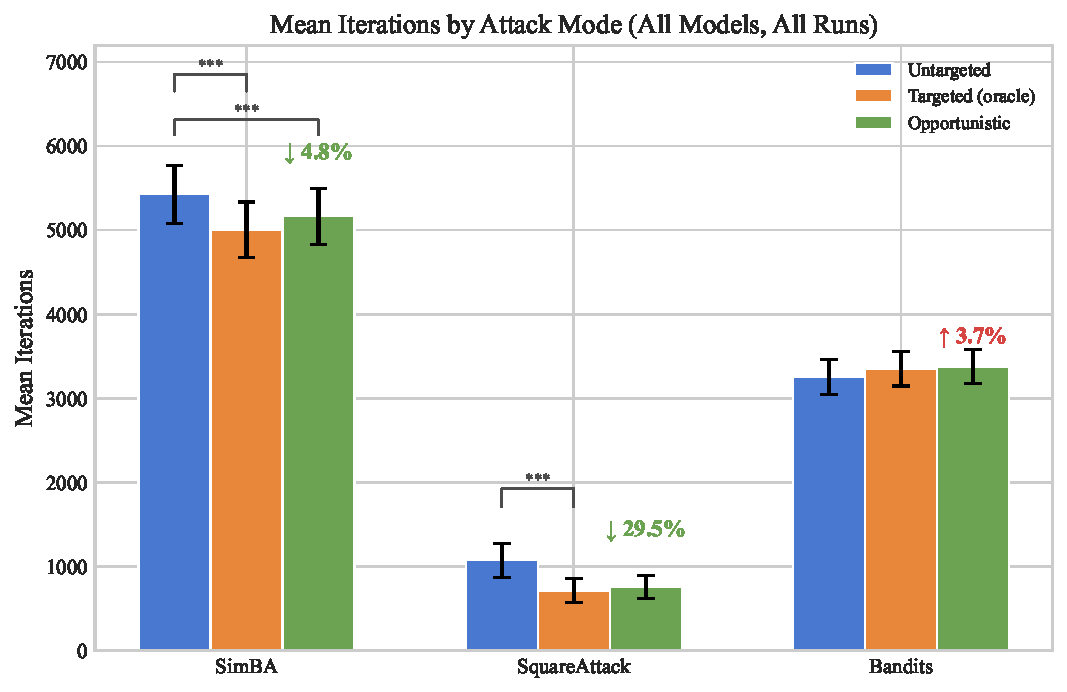
\includegraphics[width=0.98\linewidth]{fig_headline_bars.pdf}
\end{center}
\vspace{0.2cm}
\begin{center}
\begin{tabular}{@{}lccc@{}}
\toprule
Attack & Untargeted & OTS & Oracle \\
\midrule
SimBA & 67\% & \textbf{75\%} & 76\% \\
Square Attack CE & 96\% & \textbf{99\%} & 99\% \\
Bandits & 37\% & 34\% & 35\% \\
\bottomrule
\end{tabular}
\end{center}
\end{block}

\begin{block}{Query Budget View}
\begin{center}
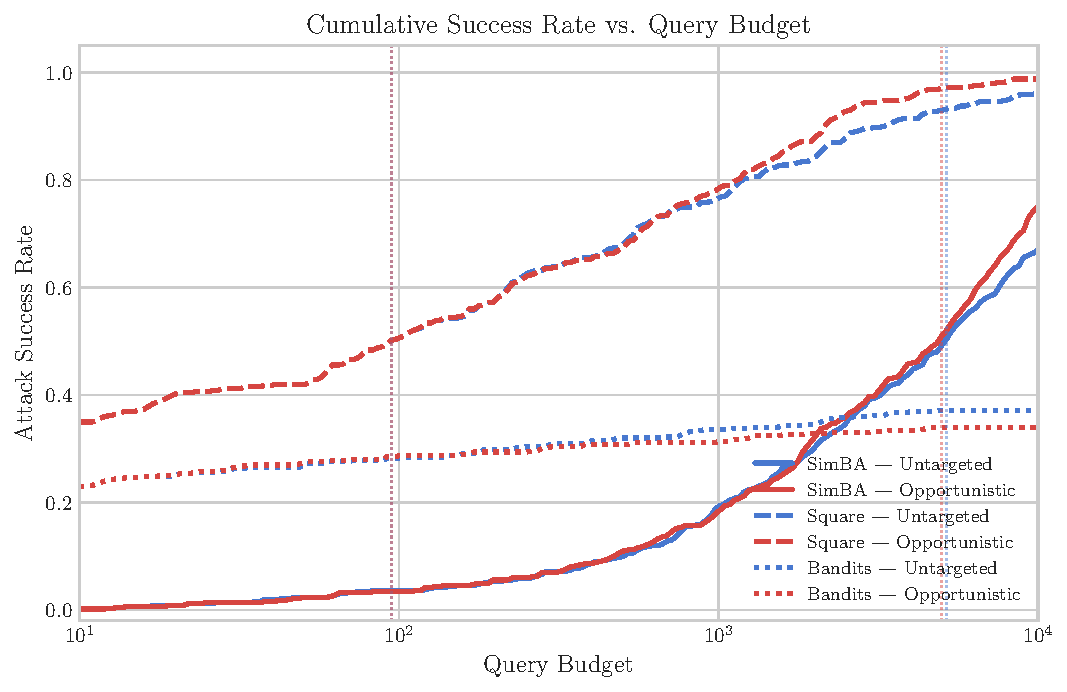
\includegraphics[width=0.98\linewidth]{fig_cdf.pdf}
\end{center}
\small
The separation is clearest for SimBA and Square Attack with CE loss. Bandits remains flat because gradient estimation already gives directional information.
\end{block}

\begin{block}{Alignment Mechanism}
\begin{center}
\includegraphics[width=0.86\linewidth]{fig_theta.pdf}
\end{center}
\small
OTS does not merely select a class label. It redirects the perturbation toward the oracle targeted direction: terminal cosine similarity rises from $0.174$ to $0.865$ on SimBA/ResNet-50.
\end{block}

\end{column}

\begin{column}{0.29\paperwidth}

\begin{block}{Where OTS Helps}
\begin{center}
\begin{tabular}{@{}p{0.38\linewidth}p{0.52\linewidth}@{}}
\toprule
Helps & Does not help \\
\midrule
SimBA probability minimization & Bandits gradient estimation \\
Square Attack with CE loss & Square Attack margin loss \\
Medium-difficulty standard models & Robust models with early-success/fail split \\
\bottomrule
\end{tabular}
\end{center}

\vspace{0.4cm}
\begin{itemize}
\tightitem
\item ResNet-50 is the strongest case: SimBA rises from 43\% to 70\% success.
\item ViT-B/16 also benefits, so the effect is about attack difficulty rather than CNN depth.
\item Easy models show floor effects because nearly every method already succeeds.
\end{itemize}
\end{block}

\begin{block}{Margin-Loss Ablation}
\begin{center}
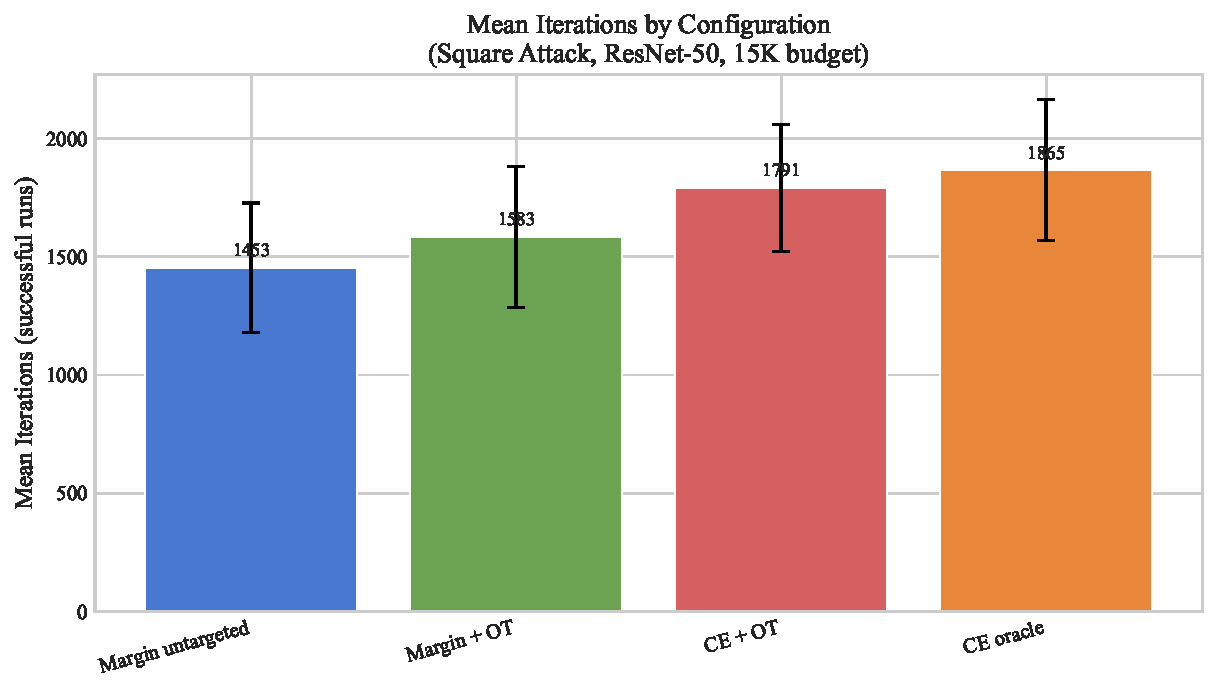
\includegraphics[width=0.98\linewidth]{fig_margin_bars.pdf}
\end{center}
\small
With CE loss, OTS restores much of the lost directionality. With margin loss, OTS is redundant.
\end{block}

\begin{block}{Target Selection Matters}
\begin{itemize}
\tightitem
\item Random targets are catastrophic: directional commitment alone is not enough.
\item Clean-image argmax nearly matches OTS for SimBA.
\item Short exploration is useful for Square Attack because patch updates disturb the class ranking more strongly.
\end{itemize}

\begin{center}
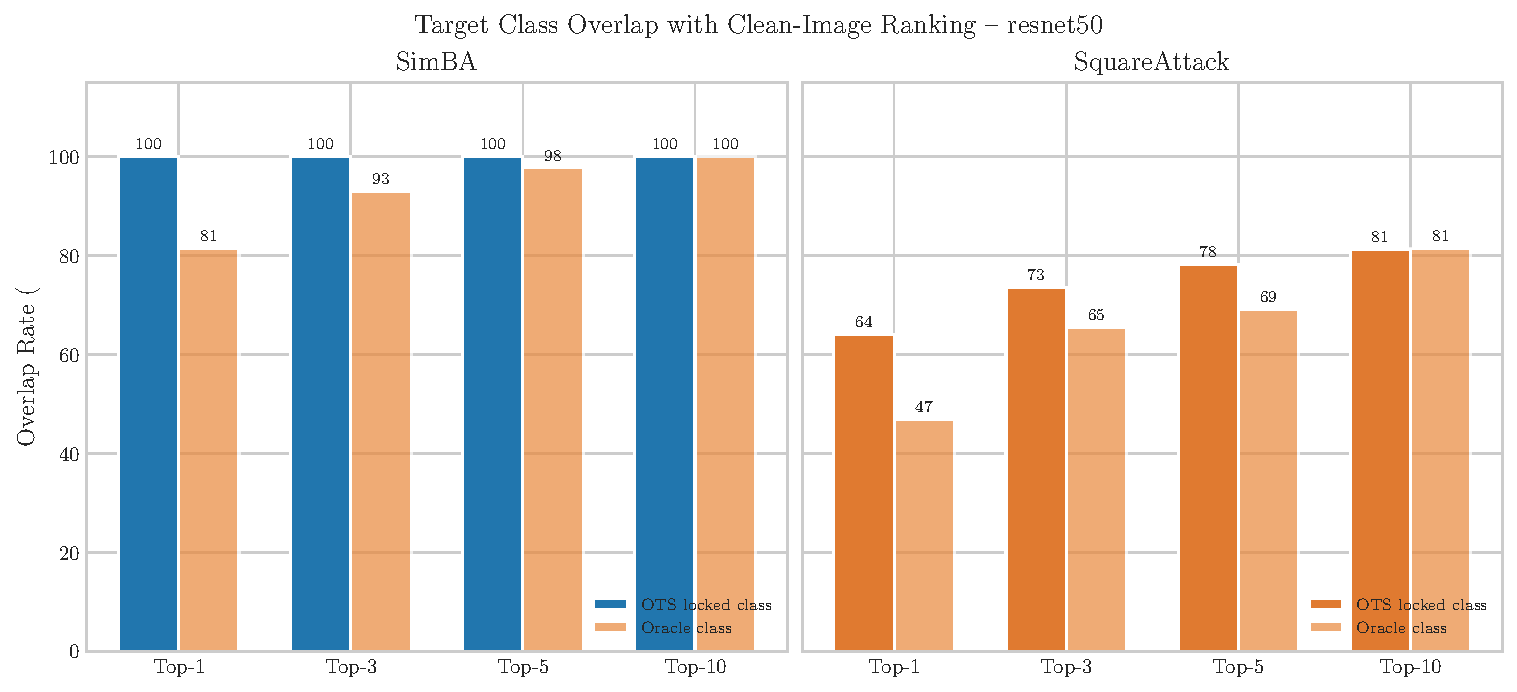
\includegraphics[width=0.92\linewidth]{fig_target_overlap.pdf}
\end{center}
\end{block}

\begin{exampleblock}{Practical Rule}
Use OTS as the default wrapper for score-based random-search attacks that optimize probability or CE objectives. Skip it for attacks already using margin loss or strong gradient-estimation priors.

\vspace{0.55cm}
\centering
{\small
\href{https://arxiv.org/abs/2605.25663}{Paper: arxiv.org/abs/2605.25663}\\
\href{https://github.com/Tariolle/opportunistic-target-selection}{Code: Tariolle/opportunistic-target-selection}
}
\end{exampleblock}

\end{column}
\end{columns}

\end{frame}
\end{document}
